\documentclass{prova}

\usepackage{amssymb}

\newcommand{\ds}{\displaystyle}

\setlength{\topmargin}{-3cm}
\setlength{\textheight}{28cm}

\professor{Prof.\@ Adriano Barbosa}
\disciplina{N\'umeros e Fun\c{c}\~oes Reais}
\avaliacao{AV2}
\curso{PROFMAT}
\data{06/07/2018}

\begin{document}
	\cabecalho{6}  % o numero 5 indica a qnt de quadros na tabela de nota
	\begin{questionario}
        \q{Dada a fun\c{c}\~ao quadr\'atica $f(x)=ax^2+bx+c$, consideremos as fun\c{c}\~oes
            afins $g(x)=mx+t$, onde $m$ \'e fixo e $t$ ser\'a escolhido
            convenientemente. Prove que existe uma \'unica escolha de $t$ para a
            qual a equa\c{c}\~ao $f(x)=g(x)$ tem uma, e somente uma, raiz $x$.
            Interprete este fato graficamente em termos dos gr\'aficos de $f$ e
            $g$.}
        \q{Seja $p(x)$ um polin\^omio do s\'etimo grau tal que $p(1) = p(2) = p(3)
            = p(4) = p(5) = p(6) = p(7) = 10$. Sabendo que $p(8)=30$, determine
            $p(-3)$.}
        \q{}
        \begin{questionario}
            \qq{Usando o gr\'afico com o qual se define geometricamente o
                logaritmo natural, mostre que \ \ \ \ \ \ $\ln(1+x)<x$ para
                todo $x>0$.  Conclua que $\ln x<x$.}
            \qq{Tomando $\sqrt{x}$ em vez de $x$ nesta \'ultima desigualdade,
                prove que para todo $x$ suficientemente grande, o quociente
                $\ds\frac{\ln x}{x}$ pode tornar-se t\~ao pequeno quanto
                desejemos.}
            \qq{Prova ainda que essa conclus\~ao \'e v\'alida para logaritmos em
                qualquer base $a>1$.}
        \end{questionario}
        \q{Sabendo que os \^angulos $C\hat{A}D$ e $C\hat{B}D$ medem, respectivamente,
            $\alpha$ e $\beta$ radianos, determine a altura $CD$ em fun\c{c}\~ao da
            medida de $AB$ e dos \^angulos $\alpha$ e $\beta$.}
        \begin{figure}[h]
            \centering
            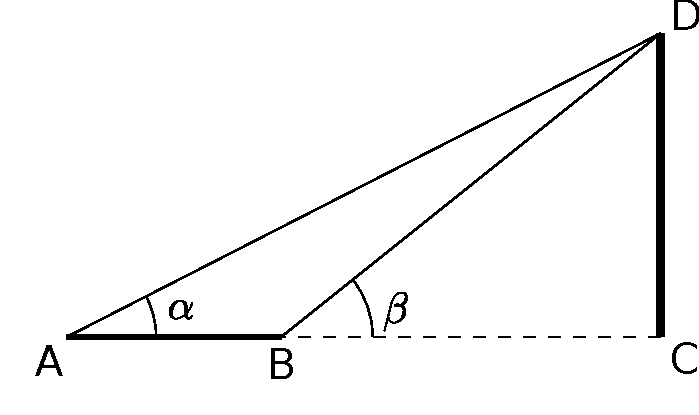
\includegraphics[width=0.3\textwidth]{q04.pdf}
        \end{figure}
        \vspace{-0.5cm}
        \q{A express\~ao $\ds M(t) = 200\ e^{-(t\ln 2)/30}$ d\'a a massa em gramas do
            c\'esio 137 que restar\'a de uma quantidade inicial ap\'os $t$ anos de
            decaimento radioativo.}
       \begin{questionario}
           \qq{Quantos gramas havia inicialmente?}
           \qq{Quantos gramas permanecem depois de 10 anos? Use, caso seja
               necess\'ario, $\ds\frac{1}{\sqrt[3]{2}} \approx 0,8$.}
           \qq{Quantos anos levar\'a para reduzir pela metade a quantidade
               inicial de c\'esio 137?}
       \end{questionario}
       \q{Um fazendeiro tem 2400m de cerca para cercar uma \'area retangular que
           margeia um rio reto. Quais devem ser as dimens\~oes da regi\~ao para que
           se tenha a maior \'area poss\'{\i}vel?}
        \begin{figure}[h]
            \centering
            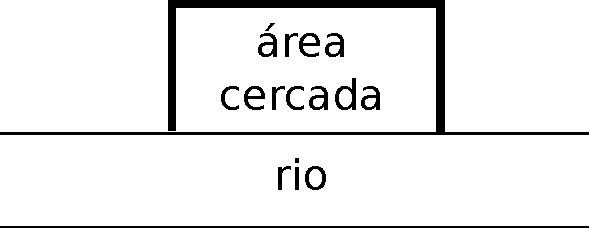
\includegraphics[width=0.3\textwidth]{q06.pdf}
        \end{figure}
        \vspace{-0.5cm}
	\end{questionario}
\end{document}
